\chapter {CellBE programming} 
\par
In this chapter will describe my experience with the CellBE platform will then follow.
Content of SDK, some usefull libraries, as well as some design patterns of CellBE programming will be described.

\section{CellBE platform development}
\par
IBM deliver SDK for development of programs fot CellBE.
It is for linux platform, in the concrete for Fedora or Red Hat distribution.
It comes in two flawors.
The official non free one which has all the features needed for development for CellBE evene for some hibrid systems and support team ready to help.
And the free one that is open to wide public and everybody can download it and start developing.
The free one does not have the tools for hibrid systems nor some tools for development in other languages than C/C++.
Wee use the free one since we develop only in C/C++ and for clean CellBE processor.

\par
Because the SDK is for Linux operation system, its user has to have already deeper knowledge about the system.
There are some bugs and parts that are not fully finished (see \ref{toolsSetup}).
Without deeper knowledge of the Linux system is impossible to react on some unexpected behaviour during installation or development phase.

\par
We have begun with SDK version 3.0 and Fedora version 8 which ware the current version of needed tools.
We have faced some obstacles and before we were able to overcome them new version of SDK (3.1) appeard.
Because we wanted to use and describe the latest tools we had to begin from scrath because new version brought new obstacles as well.

\par
The new version was declared to be compatible with new version of Fedora (9 - Sulphur) that had been released almost some time before the new version of SDK.
Previous version of SDK (3.0) was for Fedora 7 Warewolf.
We have tried all possible combinations of Fedora distributions and SDKs to find out if they are compatible with each other.
Only result from that was finding that the are not at the cost of lots of days spent on it.
The SDK is huge package of software dependent on lots of third party libraries and solutions.
They are treated differently within particular distributions and sometimes even versions of the same distribution.
So the result is not to combine versions (system, SDK nor particular libraries that the SDK components are dependent on.
Repository versions should be used, see \ref{toolsSetup}.

\par
Although there are to much of troubles when different version are combined, some efforts to get the SDK run on another distributions than Fedora were made.
But we thing the time spent is not worth the result.

\par
Finally we installed Fedora 9 Sulphur and SDK 3.1.
This combination is declared by IBM as tested.
Altough we have run into some bugs and errors.
The process of installation is described in \ref{toolsSetup}.
Installation of Fedora is omited.
For details see official site \url{http://fedoraproject.org/}.

\section {SDK content}

CellBE SDK is divided into variety of components.
Each component is contained in one or more rpm package for easy intallation purposes.
Here is list of most important available components:
\begin{enumerate}
  \item {Toolchain}
  \par
  Set of tools (compilers, linkers, ...) needed for actual code ceneration.
There are two groups of the tools.
One is for PPU and the other for SPU.

  \item {Libraries}
  \par
  IBM provides with the SDK some usefull libraries for mathematics (linear algebra, FFT, monte carlo, ...), cryptographic or runtime management.
Code of these libraries is debuged, highly optimailezed for runnig on SPEs and SIMDized.

  \item {Full system simulator}
  \par
  Program that can simulate the CellBE processor on other hardware platforms.
It is used mostly in profiling stage because simulator can simulate actual computation of a code in cycles precision.
It can of course used when programmer has not access to actuall CellBE hardware, but simulation is incredibly slow.

  \item {IDE}
  \par
  IDE is in fact verstion 3.2 of Eclipse with integration of debugging, profiling, CellBE machine management and ohter features that makes development for CellBE easier and more comfortable.
\end{enumerate}


\section{Parallel systems \& CellBE}

Parallelization depends also on type of system (hardware) where the program will be run.
There are two basic kind of paralel systems:
\begin{enumerate}
\item {shared-memory system}
\par
Is multi processor system with one shared memory which all processor can see.
Processors has to synchronize access to the memory otherwise race conditions will rise.

\item {distributed-memory system}
\par
Is system where each processor has its own private memory.
There is no need for synchronization.
\end{enumerate}

In context of parallel systems, CellBE is some kind of hybrid system.
SPEs matches the distributed-memory system (due to private local stores) while PPE is shared-memory system.
Sometimes called heterogenous multi-core, with distributed memory.
Because CellBE processors can be gathered into bigger units (e.g. blade server, with two CellBE chips) they can be viewed as either 16 + 2 cores in SMP mode or two non-uniform memory access machines connected together.
Programmer has then decide which view of the CellBE processor is better for the solved problem.

\section{CellBE programming models}

Implementation of paralel algorithms rely on paralel programming model.
That is a set of software technologies (such as programming languages extension, special compilers, libraries) through that actual paralelism is achieved.
So another decision that programmer has to make is to choose a programming model or mixture of them that will best fit for the solved problem.

For CellBE there are variety of parallel programming models.
They differ from each other in view of the hardware (hardware model) and thus how many action (such as task distribution management, data distribution management, synchronization) are performed implicitely by the model.
 The most abstract ones can perform many action implicit (i.e. ease of implementation) but at cost there can be no performance tunning done.
 And on the other hand the most concrete one see the CellBE with all the details and actions performed can be tunned and performed explicitely in way application requires.

There are some models that are determined only for CellBE platform and are contained in SDK.
 While there are another models (such as MPI, openMP) that are compatible but they would expose only PPE, will not further decribed.

List of the programming models (frameworks) follows in order from most concrete to most abstract:
\begin{enumerate}
\item {libspe2}
\par
Offers features such as SPE context management (creating, running, scheduling, and deleting), DMA primitives for data transfer, mailboxes, signal, events, and synchronization functions for PPE to SPE and SPE to SPE dialogs. 

\item {Data Communication and Synchronization - DaCS}
\par
Defines program entity for PPE or SPE (HE - host element program for PPE and AE - accelerator element program for SPE).
Provides some services for that programs.
These are resource and process management, where an HE manipulates its AEs.
Group management, for defining groups within which synchronization events like barriers can happen.
Message passing by using send and receive primitives etc.

\item {Accelerated Library Framework - ALF}
\par
ALF defines ALF-task as another entity that perform computationaly intensive parts of a program.
The idea is to have the host program split the work into multiple independent pieces, which are called work blocks.
They are described by a computational kernel, the input and the output data. Programming with ALF is divided into two side.
The host and the accelerator one.
On the accelerator side, the programmer only has to code the computational kernel, unwrap the input data, and pack the output data when the kernel finishes.
The ALF offer clear separation between host accelerator sides of program parts.
Providing the following services (from programmers view for free): work blocks queue management, load balancing between accelerators, transparent DMA transfers, ...

\end{enumerate}

Choosing a framework is important decision of writing CellBE application.
 It should be considered enough.

\section {CellBE paralelism levels}

The CellBE processor offers many opportunities for parallel processing.
That is because it is composed of and can be compound to heterogenous elements.
 Levels are:
\begin{enumerate}
\item server level
\par
In a hybrid environment at the cluster level using MPI or some sort of grid computing middleware.

\item CellBE chips level
\par
In case there are more in the machine (e.g. blade server with two CellBEs). Using ALF or DaCS for hybrid.

\item SPE level
\par
Inside the CellBE chip offloading intensive parts of code to SPE, using libspe, ALF, DaCS.

\item SIMD instruction level
\par
Instruction that process more data in parallel. Using leanguage intrinsic.
\end{enumerate}

\section{Computation configurations}

\par
Because of heterogenous nature of CellBE and its PPU \& SPEs processing elements some different computation configuration are used.
 They differ in usage of SPUs and hase its own pros and cons:
\begin{enumerate}
\item Streaming configuration
\par
All SPE serves as a stream processor (see figure \ref{fg:streamingModel}).
They run exact same code expecting the same type of data and producing also the same of data type.
This configuration is well suited for some streaming application for example filters where there is still the same type of data on input.
No SPU context need not to be switched that save according time.
One disadvantage is that configuration is static.

\begin{figure}
    \centering
    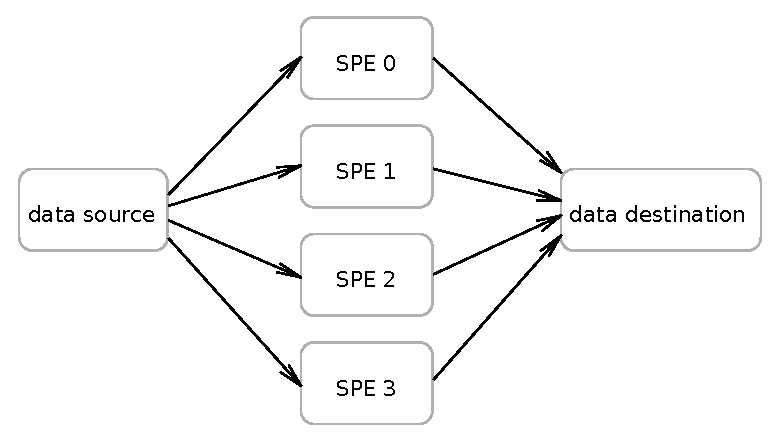
\includegraphics[width=0.7\textwidth]{data/streamingModel}
    \caption[Streaming SPE configuration]{All SPE run the same code creating farm of processor that process same type of data.}
    \label{fg:streamingModel}
\end{figure}

\item Pipeline configuration
\par
SPE server as stages of an pipeline (see figure \ref{fg:pipelineModel}).
Data are passed through from one to other of the SPEs.
The SPE to SPE transfer are faster than SPE to PPE so this can be benefit.
The configuration is also static which means no SPU context switch.

\begin{figure}
    \centering
    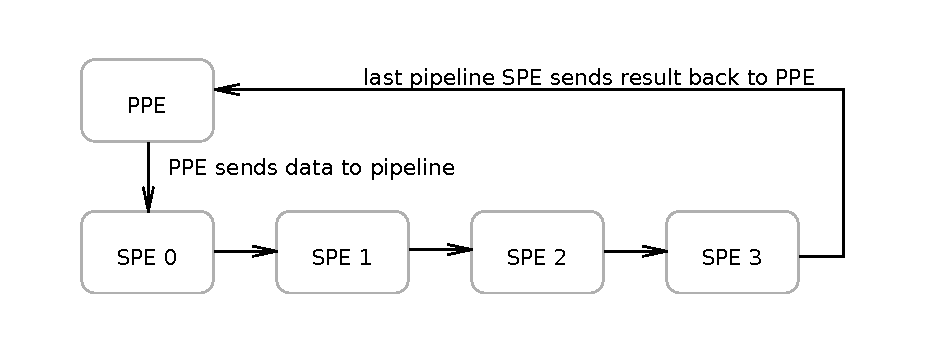
\includegraphics[width=0.7\textwidth]{data/pipelineModel}
    \caption[Pipeline SPE configuration]{SPE creates pipeline. Each spe represent one stage of that pipeline. Data are transferred only via SPE to SPE DMA transfers benefiting the speed of bus.}
    \label{fg:pipelineModel}
\end{figure}

\item PPU centric
\par
This configuration is common approach with CellBE.
Program runs on PPE (see figure \ref{fg:PPUCentricModel})and only selected, highly demanding computational kernels (hotspots) are offloaded to SPEs.
This method is the easiest from a program development perspective because it limits the scope of source code changes and does not require much re-engineering at the application logic level.
One disadvantage is dynamic changes of SPE contexts that is quite expensive opertation.

\begin{figure}
    \centering
    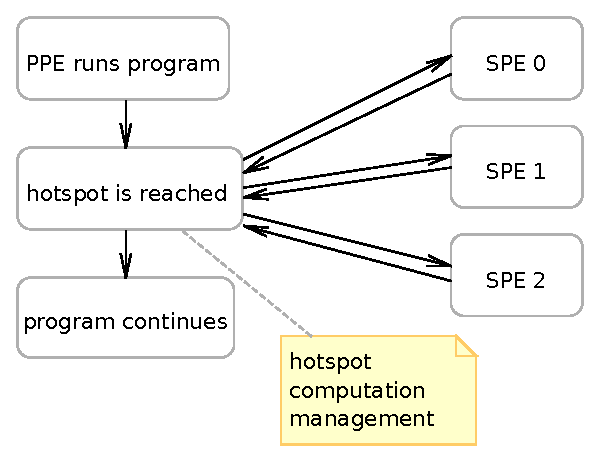
\includegraphics[width=0.7\textwidth]{data/PPUCentricModel}
    \caption[PPU centric configuration]{Program is run on PPE and only hotspots are offloaded to SPEs.
 Offloading means managing SPE context creation and loading as well as managing data transfer and synchronization between PPE and SPUs}
    \label{fg:PPUCentricModel}
\end{figure}

\item SPE server
\par
Another configuration is to have server-like programs running on SPEs that sits and waits offering some functionality.
 This is requires the code to be small enough to fit into the SPU local store along with processed data.

\end{enumerate}

\section {Building for CellBE}
\par
Actual building is done using selected toolchain.
 But there is difference between management of code building for PPU and SPU.
 It is caused by difference of actual code usage.
While PPU code resides in central memory (just like in common architectures) SPU code is loaded into SPE dynamically and shall be somehow separated.
 It is similar to shader programs for graphic accelerators.
They are also loaded into appropriate processors when they are needed and live separated (in form of files).

//TODO obrazek

\par
There are two options for SPE code management.
 One is to build shared library and load it explicitly when it is used.
 Another way is to build a static library and include it into PPU executable.
 This inclusion is called embeding and is performed with extra tool from toolchain.
The SPU program is then referenced as special extern structure direct from PPU code (instead of performing some shared libraries loading).
 Both ways has its pros but even cons which are the same as with shared vs. static libraries on other platforms.


\section {Process of porting application for CellBE}

\par
The most common process of porting an application for CellBE system (figure \ref{fg:appPorting}) begins with locatlization of compute intensive parts, hotspots (by profiling of the application on PPE).
 Hotspot computation is then moved to the SPEs.
 Then the SIMDation (i.e. rewriting scalar code into vectorised to be able to use SIMD instruction) of the hotspots and data movement tunnig can be performed until satisfactory performance is obtained.
 The whole process is repeated for every single hotspot.

\begin{figure}
    \centering
    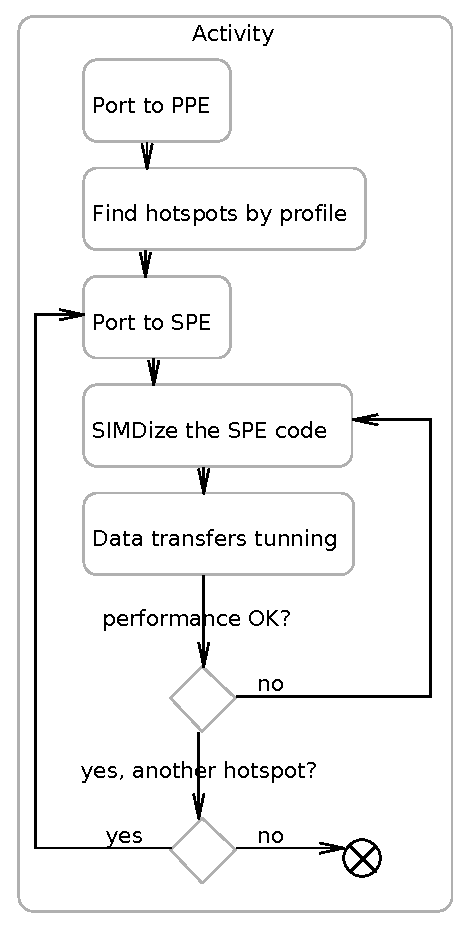
\includegraphics[height=\textwidth]{data/portingCycle}
    \caption[Application for CellBE porting process]{Diagram shows all stages of the process and loops for better performance tunnig and other hotspots}
    \label{fg:appPorting}
\end{figure}
